\documentclass{cours}

\title{Calcul Intégral}

\begin{document}
    \maketitle{16}
    
    \begin{Gpartie}{Notion d'Intégrale} 
        \begin{Spartie}{Aire sous la Courbe et Intégrale} 
            \begin{SSpartie}{Défintion} 
                Soit $f$ une fonction \emph{continue et positive} sur un intervalle $\big[a~;b\big]~\left(a\leq b\right)$ et $\mathcal{C}$ sa courbe représentative dans un repère orthogonal.

                L'aire délimitée par $\mathcal{C}$, l'axe des abscisses et les droites d'équation $x=a$ et $x=b$ est l'intégrale de $f$ sur $\big[a~;b\big]$, et se note : \[\int_a^b f(t)\dt\]
            \end{SSpartie}
            \begin{SSpartie}{Remarques} 
                $\int_a^b f(t)\dt$ se lit \og intégrale de $a$ à $b$ de $f$ de $t~\dt$ \fg{} \\ ou \og somme de $a$ à $b$ de $f$ de $t~\dt$ \fg{}.

                $\int_a^b f(t)\dt$ se note indifféremment $\int_a^b f(x)\dx$

                $\int_a^b f(t)\dt$ se mesure en unité d'aire ($u.a.$). Où $1~u.a.$ est l'aire du rectangle de base (1 sur 1).
            \end{SSpartie}
            \begin{SSpartie}{Remarque} 
                Dans le cas d'une fonction continue de signe quelconque, $\int_a^b f(t)\dt$ est une aire algébrique entre la courbe, l'axe des abscisses et les droites d'équation $x=a$ et $x=b$.

                Par convention, on compte positivement les aires lorsque $\mathcal{C}$ est au dessus de l'axe des abscisses et négativement lorsqu'elle est en dessous.
            \end{SSpartie}
        \end{Spartie}
        \pagebreak
        \begin{Spartie}{Dérivabilité de la Fonction Aire} 
            \begin{SSpartie}{Théorème} 
                Soit $f$ une fonction continue et positive sur $\big[a~;b\big]~\left(a\leq b\right)$

                Alors, la fonction $\Phi:x\mapsto\int_a^xf(t)\dt$ est dérivable sur $\big[a~;b\big]$ et : \[\Phi'=f\qquad\text{($\Phi$ est une primitive de $f$)}\]
                \begin{SSSpartie}{Démonstration \big($f$ croissante\big)} 
                    Soit $x_0\in\big[a~;b\big]$ et $h\neq 0$ tel que $x_0+h\in\big[a~;b\big]$. Notons $\mathcal{C}$ la courbe représentative de $f$.

                    \begin{center}
                        \begin{tikzpicture}[scale=0.8]
                            \begin{axis}[
                                xmin=-0.25, xmax=4.25,
                                ymin=-0.3, ymax=3.75,
                                xtick=\empty,
                                ytick=\empty,
                                domain=0.5:3.75
                            ]
                                \addplot[blue, very thick]{e^(0.3*\x)};
                                \draw[dashed, thick] (0.5,0) node[label={[label distance=-6pt]below:$a$}] {} -- (0.5,1.16) node[dot] {};
                                \draw[dashed, thick] (3.75,0) node[label={[label distance=-7.5pt]below:$b$}] {} -- (3.75,3.08) node[dot] {};
                                % \draw[pattern=north west lines] (1.5,1.57) -- (1.5,0) -- (2.5,0) -- (2.5,1.57) -- cycle;
                                \draw[black!60!green, pattern=north west lines] (1.5,1.57) rectangle (2.5,0);
                                \draw[red,pattern=north west lines] (1.5,1.57) rectangle (2.5,2.12);
                                \node[anchor=north,inner sep=2pt] at (1.5,0) {$x_0$};
                                \node[anchor=north,inner sep=2pt] at (2.5,0) {$x_{0+h}$};

                            \end{axis}
                        \end{tikzpicture}
                        \parbox{\linewidth}{\captionof{figure}{\centering Encadrement de la Fonction $\Phi$}}
                    \end{center}

                    Étudions $\lim\limits_{h\to0}\dfrac{\Phi\left(x_0+h\right)-\Phi\left(x_0\right)}{h}$

                    $\Phi\left(x_0+h\right)-\Phi(x_0)$ est l'aire sous la courbe entre $x_0$ et $x_0+h$.

                    On encadre cette aire par les aires des deux rectangles de largeur $\lvert h\rvert$ et de hauteur $f(x_0)$ (en vert) et $f(x_0+h)$ (en rouge)

                    \begin{itemize}
                        \item Si $h>0$, et comme $f$ est croissante :
                        
                        $\begin{aligned}[t]
                            &\quad h\times f(x_0)\leq\Phi\left(x_0+h\right)-\Phi(x_0)\leq h\times f(x_0+h) \\
                            \iff&\quad f(x_0)\leq \frac{\Phi\left(x_0+h\right)-\Phi(x_0)}{h}\leq f(x_0+h) 
                        \end{aligned}$

                        \item Si $h<0$ alors la largeur est $-h$ :
                        
                        $\begin{aligned}[t]
                            &\quad -h\times f(x_0+h)\geq\Phi(x_0)-\Phi(x_0+h)\geq -h\times f(x_0) \\
                            \iff&\quad f(x_0+h)\leq\frac{\Phi\left(x_0+h\right)-\Phi(x_0)}{h}\leq f(x_0)
                        \end{aligned}$
                    \end{itemize}
                    Or $f$ est continue, donc $\lim\limits_{h\to0}f(x_0+h)=f(x_0)$

                    Donc, d'après le théorème des gendarmes : \[\lim\limits_{h\to0}\frac{\Phi\left(x_0+h\right)-\Phi(x_0)}{h}=f(x_0)\quad\square\]

                    Ainsi, $\Phi$ est dérivable en $x_0$ et $\Phi'(x_0)=f(x_0)$.

                    Ce résultat est vrai pour tout $x_0\in I$, donc $\Phi$ est dérivable sur $I$ et $\Phi'=f$.
                \end{SSSpartie}
            \end{SSpartie}
            \begin{SSpartie}{Rappel Théorème} 
                Soit $f$ une fonction continue sur $I$ et $\Phi$ une primitive de $f$ sur $I$.

                Alors, $f$ admet une infinité de primitives sur $I$ et toute primitive $F$ de $f$ est définie par $F(x)=\Phi(x)+k,~k\in\mathbb{R}$.
            \end{SSpartie}
            \begin{SSpartie}{Conséquence} 
                Soit $f$ une fonction continue et positive sur $\big[a~;b\big]$.

                Le premier théorème prouve l'existence d'une primitive $\Phi$ de $f$ sur $\big[a~;b\big]$, définie par $\Phi(x)=\int_a^xf(t)\dt$.

                Ainsi, $\int_a^b f(t)\dt=\Phi(b)$

                Et d'après le deuxième théorème (lien entre deux primitives), quelle que soit $F$,~la primitive de $f$, il existe un réel $k$ tel que $F=\Phi+k$. \\ Donc, $F(a)=\Phi(a)+k=k$ car $\Phi(a)=\int_a^af(t)\dt=0$.

                Ainsi, $\Phi(b)=F(b)-k=F(b)-F(a)$

                Or $\Phi(b)=\int_a^b f(t)\dt$
                
                Donc, quelle que soit la primitive $F$ de $f$ : \[\int_a^b f(t)\dt=F(b)-F(a)\]
            \end{SSpartie}
            \begin{SSpartie}{Remarque} 
                On note : \[\int_a^b f(t)\dt=\big[F(t)\big]_a^b=F(b)-F(a)\]
            \end{SSpartie}
            \begin{SSpartie}{Exemples} 
                \begin{itemize}
                    \item $\displaystyle \int_0^1\me^x\dx=\big[\me^x\big]_0^1=\me^1-\me^0=\me-1$
                    \item $\displaystyle \int_0^2t^2\dt=\Bigg[\frac{t^3}{3}\Bigg]_0^2=\frac{2^3}{3}-\frac{0^3}{3}=\frac{8}{3}$
                \end{itemize}
            \end{SSpartie}
        \end{Spartie}
    \end{Gpartie}
    \begin{Gpartie}{Intégrale d'une Fonction Continue} 
        \begin{Spartie}{Extension de la Notion d'Intégrale} 
            On a défini l'intégrale d'une fonction $f$ continue et positive sur un intervalle $\big[a~;b\big]~\left(a\leq b\right)$, et on a vu que si $F$ est une primitive de $f$ sur $\big[a~;b\big]$ : \[\int_a^b f(t)\dt=F(b)-F(a)\]

            On admet que cette formule peut être étendue au cas d'une fonction continue de signe quelconque, quelles que soient les bornes $a$ et $b$ de l'intégrale.

            \begin{SSpartie}{Définition} 
                Soit $f$ une fonction continue sur un intervalle $I$ et soit $F$ une primitive de $f$ sur $I$. Si $a$ et $b$ sont deux réels quelconques de $I$, l'intégrale de $f$ entre $a$ et $b$ s'écrit : \[\int_a^b f(t)\dt=\big[F(t)\big]_a^b=F(b)-F(a)\]
            \end{SSpartie}
            \begin{SSpartie}{Exemples} 
                \begin{itemize}
                    \item   
                    $\begin{aligned}[t]
                        \int_{-4}^{-2}\left(\frac{1}{t^2}-3\right)\dt=\Bigg[\frac{-1}{t}-3t\Bigg]_{-4}^{-2}&=\frac{-1}{(-2)}-3\times(-2)-\left(\frac{-1}{(-4)}-3\times(-4)\right)  \\
                        &=\frac{1}{2}+6-\frac{1}{4}-12 \\
                        &=\frac{-23}{4}
                    \end{aligned}$

                    \item 
                    $\begin{aligned}[t]
                        \int_\frac{1}{2}^1\left(\frac{1}{t}-t^2\right)\dt=\Bigg[\ln\,(t)-\frac{t^3}{3}\Bigg]_\frac{1}{2}^1&=\ln\,(1)-\frac{1}{3}-\left(\ln\,\left(\tfrac{1}{2}\right)-\frac{\left(\frac{1}{2}\right)^3}{3}\right) \\
                        &=\frac{-1}{3}+\ln\,(2)+\frac{1}{24} \\
                        &=\frac{7}{24}+\ln\,(2)
                    \end{aligned}$
                    \item 
                    $\begin{aligned}[t]
                        \int_{-2}^1t\dt=\Bigg[\frac{t^2}{2}\Bigg]_{-2}^1&=\frac{1^2}{2}-\frac{(-2)^2}{2} \\
                        &=\frac{3}{2}
                    \end{aligned}$
                \end{itemize}
            \end{SSpartie}
            \pagebreak
            \begin{SSpartie}{Conséquences} 
                \begin{itemize}
                    \item $\displaystyle\int_a^af(t)\dt=0\quad\big(=F(a)-F(a)\big)$
                    \item $\displaystyle\int_b^af(t)\dt=F(a)-F(b)=-\int_a^b f(t)\dt$
                \end{itemize}
            \end{SSpartie}
        \end{Spartie}
        \begin{Spartie}{Linéarité de l'Intégrale} 
            \begin{SSpartie}{Théorème} 
                Soient $f$ et $g$ deux fonctions continues sur $I$ et soit $\lambda$ un réel. Pour tous réels $a$ et $b$ de $I$ : \[\int_a^b\left(f+g\right)(t)\dt=\int_a^b f(t)\dt+\int_a^bg(t)\dt\] \[\int_a^b\lambda f(t)\dt=\lambda\int_a^b f(t)\dt\]
                \begin{SSSpartie}{Démonstration} 
                    Soient $F$ et $G$ des primitives de $f$ et $g$. Alors $F+G$ et $\lambda F$ sont des primitives de $f+g$ et $\lambda f$ respectivement.
                    \begin{itemize}
                        \item 
                        $\begin{aligned}[t]
                            \int_a^b\left(f+g\right)(t)\dt&=\left(F+G\right)(t)-\left(F+G\right)(t) \\
                            &=F(b)+G(b)-F(a)-G(a) \\
                            &=F(b)-F(a)+G(b)-G(a) \\
                            &=\int_a^b f(t)\dt+\int_a^b g(t)\dt
                        \end{aligned}$

                        \item $\begin{aligned}[t]
                            \int_a^b\lambda f(t)\dt&=\lambda F(b)-\lambda F(a) \\
                            &=\lambda\left(F(b)-F(a)\right) \\
                            &=\lambda\int_a^b f(t)\dt
                        \end{aligned}$
                    \end{itemize}
                \end{SSSpartie}
            \end{SSpartie}
        \end{Spartie}
        \pagebreak
        \begin{Spartie}{Relation de Chasles} 
            \begin{SSpartie}{Théorème} 
                Soit $f$ une fonction continue sur un intervalle $I$. Quels que soient les réels $a$, $b$ et $c$ appartenant à $I$ : \[\int_a^c f(t)\dt=\int_a^b f(t)\dt+\int_b^cf(t)\dt\]
                \begin{SSSpartie}{Démonstration} 
                    Soit $F$ une primitive de $f$.

                    $\begin{aligned}[t]
                        \int_a^c f(t)\dt&=F(c)-F(a) \\
                        &=F(c)-F(b)+F(b)-F(a) \\
                        &=\int_a^b f(t)\dt+\int_b^c f(t)\dt
                    \end{aligned}$
                \end{SSSpartie}
            \end{SSpartie}
            \begin{SSpartie}{Remarque} 
                Dans le cas où $f$ est positive et $a\leq b\leq c$, la relation de Chasles traduit l'additivité des aires de deux domaines adjacents.
            \end{SSpartie}
            \begin{SSpartie}{Exemple} 
                Intégrale d'une fonction définie par morceaux : \[\int_{-2}^5f(x)\dx\quad\text{où}\quad f:x\mapsto\lvert x\rvert-2\qquad\lvert x\rvert\begin{cases}x\geq0:x\\x<0:-x\end{cases}\]

                $\begin{aligned}[t]
                    \int_{-2}^5f(x)\dx &= \int_{-2}^0f(x)\dx+\int_0^5f(x)\dx \\
                    &= \Bigg[\frac{-x^2}{2}-2x\Bigg]_{-2}^0+\Bigg[\frac{x^2}{2}-2x\Bigg]_0^5 \\
                    &= 0-2+\frac{5}{2}-0=\frac{1}{2} 
                \end{aligned}$
            \end{SSpartie}
        \end{Spartie}
        \pagebreak
        \begin{Spartie}{Positivité et Ordre} 
            \begin{SSpartie}{Théorème} 
                Soit $f$ une fonction continue sur $I$, et $a$ et $b$ deux réels de $I$ tels que $a\leq b$

                Si $\forall t\in I,~f(t)\geq0$ : \[\int_a^b f(x)\dt\geq0\]
                \begin{SSSpartie}{Démonstration} 
                    Dans le cas d'une fonction continue et positive sur $\big[a~;b\big],~\int_a^b f(t)\dt$ est l'aire sous la courbe représentative de $f$ entre $a$ et $b$, elle est positive.
                \end{SSSpartie}
            \end{SSpartie}
            \begin{SSpartie}{Théorème} 
                Soient $f$ et $g$ deux fonctions continues sur un intervalle $I$ et $a$ et $b$ deux réels tels que $a\leq b$

                Si $\forall t\in I,~f(t)\leq g(t)$ : \[\int_a^b f(t)\dt\leq\int_a^bg(t)\dt\]
                \begin{SSSpartie}{Démonstration} 
                    $g-f$ est positive sur $I$ donc : 

                    $\begin{aligned}[t]
                        &\quad\int_a^b\left(g-f\right)(t)\dt\geq 0 \\
                        \iff&\quad\int_a^b g(t)\dt-\int_a^b f(t)\dt\geq 0 \\
                        \iff&\quad\int_a^b f(t)\dt\leq\int_a^b g(t)\dt
                    \end{aligned}$
                \end{SSSpartie}
            \end{SSpartie}
        \end{Spartie}
    \end{Gpartie}
    \pagebreak
    \begin{Gpartie}{Valeur Moyenne d'une Fonction Continue} 
        \begin{Spartie}{Valeur Moyenne} 
            \begin{SSpartie}{Définition} 
                Soit $f$ une fonction continue sur un intervalle $\big[a~;b\big]$, avec $a<b$, la valeur moyenne de la fonction $f$ sur $\big[a~;b\big]$ est le nombre $\mu$ défini par : \[\mu=\frac{1}{b-a}\int_a^b f(t)\dt\]
            \end{SSpartie}
            \begin{SSpartie}{Remarque} 
                Interprétation dans le cas d'une fonction positive : \[\int_a^b f(t)\dt=\mu(b-a)\]
                \begin{center}
                    \begin{tikzpicture}
                        \begin{axis}[
                            xmin=-0.5, xmax=5,
                            ymin=-0.5, ymax=5,
                            xtick=\empty,
                            ytick=\empty,
                            domain=1:4
                        ]
                            \addplot[name path=a,blue, very thick]{0.7*(\x-2.5)^3-\x+5.5};
                            \draw (0,3.06) node[anchor=east] {$\mu$} -- (5,3.06);
                            \node[anchor=north] at (2.5,0) {$b-a$};

                            \path[name path=axis] (axis cs:1,0) -- (axis cs:4,0);

                            \addplot [
                                thick,
                                color=blue,
                                fill=blue, 
                                fill opacity=0.2
                            ]
                            fill between[
                                of=a and axis,
                                soft clip={domain=1:4},
                            ];

                        \end{axis}
                    \end{tikzpicture}
                    \hspace{0.5cm}
                    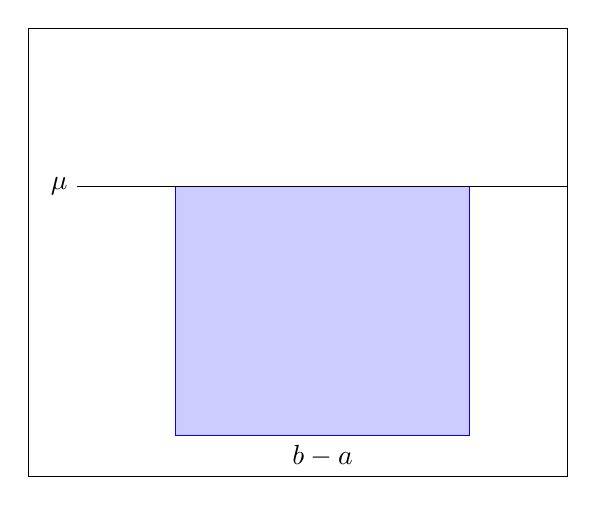
\begin{tikzpicture}
                        \begin{axis}[ 
                            xmin=-0.5, xmax=5,
                            ymin=-0.5, ymax=5,
                            xtick=\empty,
                            ytick=\empty
                        ]
                            \draw[color=blue, fill=blue, fill opacity=0.2] (1,0) rectangle (4,3.06);
                            \draw (0,3.06) node[anchor=east] {$\mu$} -- (5,3.06);
                            \node[anchor=north] at (2.5,0) {$b-a$};
                        \end{axis}
                    \end{tikzpicture}
                    \parbox{\linewidth}{\captionof{figure}{\centering Interprétation Graphique de la Valeur Moyenne pour une Fonction Positive}}
                \end{center}

                $\mu$ est la hauteur du rectangle de largeur $b-a$ dont l'aire est la même que celle du domaine situé en sous la courbe $\mathcal{C}_f$ entre $a$ et $b$.
            \end{SSpartie}
        \end{Spartie}
        \pagebreak
        \begin{Spartie}{Inégalité de la Moyenne (encadrement \og grossier \fg{} de l'intégrale)} 
            \begin{SSpartie}{Théorème} 
                Soit $f$ une fonction continue sur $\big[a~;b\big]$, $a<b$ et $m$ et $M$ deux réels tels que $\forall x\in\big[a~;b\big],~m\leq f(x)\leq M$

                On a donc : \[m(b-a)\leq\int_a^b f(t)\dt\leq M(b-a)\]
                \begin{SSSpartie}{Démonstration} 
                    $\begin{aligned}[t]
                        &\quad m\leq f(t)\leq M \\
                        \iff&\quad\big[mx\big]_a^b\leq\int_a^b f(t)\dt\leq \big[Mx\big]_a^b\quad\text{(positivité de l'intégrale)} \\
                        \iff&\quad m(b-a)\leq\int_a^b f(t)\dt \leq M(b-a)\quad\square
                    \end{aligned}$
                \end{SSSpartie}
            \end{SSpartie}
            \begin{SSpartie}{Remarques} 
                Interprétation en cas d'une fonction positive : L'aire de la courbe $\mathcal{C}_f$ est comprise entre les aires des rectangles de longueur $b-a$ et de hauteurs respectives $m$ et $M$.
                
                Encadrement de la valeur moyenne :

                $\begin{aligned}[t]
                    &\quad m(b-a)\leq\int_a^b f(t)\dt \leq M(b-a) \\
                    \iff&\quad m\leq\frac{\int_a^b f(t)\dt}{b-a}\leq M \\
                    \iff&\quad m\leq\mu\leq M
                \end{aligned}$
            \end{SSpartie}
        \end{Spartie}
    \end{Gpartie}
    \pagebreak
    \begin{Gpartie}{Intégration par Parties} 
        \begin{Spartie}{Propriété} 
            Soient $u$ et $v$ deux fonction dérivables telles que leurs dérivées $u'$ et $v'$ sont continues sur un intervalle $\big[a~;b\big]$. Alors : \[\int_a^b u(x)v'(x)\dx=\big[u(x)v(x)\big]_a^b-\int_a^b u'(x)v(x)\]
            \begin{SSpartie}{Démonstration} 
                Pour toute fonction $f$ dérivable dont la dérivée $f'$ est continue sur $\big[a~;b\big]$ :

                $\displaystyle \int_a^b f'(x)\dx=f(b)-f(a)=\big[f(x)\big]_a^b$\quad En effet, $f$ est un primitive de $f'$.

                Ainsi : \[\displaystyle \int_a^b (u v)'(x)\dx=\big[u(x)v(x)\big]_a^b\]

                Or : 
                \[\begin{aligned}[t]
                    \int_a^b (u v)'(x)\dx &= \int_a^b u'(x)v(x)+u(x)v'(x)\dx \\
                    &=\int_a^b u'(x)v(x)\dx + \int_a^b u(x)v'(x)\dx\quad\text{(linéarité)}
                \end{aligned}\]

                On a donc :
                \[\begin{aligned}[t]
                    &\quad\big[u(x)v(x)\big]_a^b = \int_a^b u'(x)v(x)\dx + \int_a^b u(x)v'(x)\dx \\
                    \iff&\quad\int_a^b u(x)v'(x)\dx=\big[u(x)v(x)\big]_a^b-\int_a^b u'(x)v(x)\dx\quad\square
                \end{aligned}\]
            \end{SSpartie}
        \end{Spartie}
    \end{Gpartie}
\end{document}